\documentclass{article}
\usepackage{custom}
\usepackage{shortex}
\usepackage{tikz}
\title{CIS-7 Unit 3 In Class Work}

\setcounter{section}{3}

\begin{document}

\maketitle
\pagebreak

\begin{enumerate}
	\item $A\in B$
	\item $V\in T$
	\item $\begin{Bmatrix}
			1 & 2 & 3 & 4 & 5
		\end{Bmatrix}$
	\item $\begin{Bmatrix}
			1 & 2 & 3 & 4 & 5 & 6 & 7 & 8 & 9
		\end{Bmatrix}$
	\item $F = \emptyset $
	\item 
		\begin{enumerate}
			\item Get the cardinality of the set. If they aren't the same, they are not equal.
			\item Sort each set.
			\item Check element by element for equality, if one doesn't match then they are not the same.
		\end{enumerate}

	\item $
		\{R \in T \mid |R| > 7\} = \{3, 7, 10, 14, 17\}
		$

	\item 
		\begin{enumerate}
			\item $\cbra{x \mid x \in  \ints, Y^{3}>3}$
			\item $Y=\cbra{x \mid x \in \ints, Y^{2}<100}$ 
			\item $\cbra{Y \in \ints \mid Y^{2} < 100}$ 
			\item $\cbra{S \mid S = 9Y, Y \in \nats}$
		\end{enumerate}

	\item 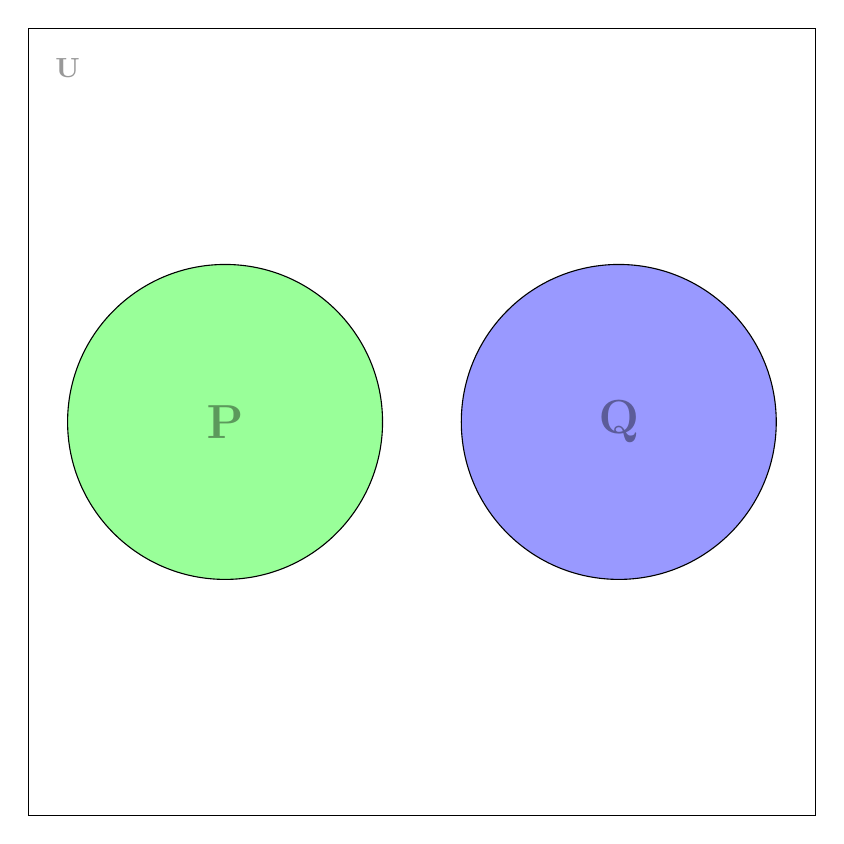
\begin{tikzpicture}
			\begin{scope}[fill opacity=.4]
				\draw (-5, 5) rectangle (5, -5);
				\node at (-4.5, 4.5) {\textbf{U}};

				\draw[fill=green, draw = black] (-2.5,0) circle (2);
				\draw[fill=blue, draw = black] (2.5,0) circle (2);
				\node at (-2.5,0) {\LARGE\textbf{P}};
				\node at (2.5,0) {\LARGE\textbf{Q}};
			\end{scope}
		\end{tikzpicture} 
	\item \begin{enumerate}
			\item True. 
			\item False.
			\item $X\subset Y$ $X\ne Y$ Not strictly true, if $X=Y$ $X\subset Y$
		\end{enumerate}
	\item \begin{enumerate}
			\item $\cbra{10, 20, 30, 40, 50, 60, 70} $
			\item $\cbra{10, 20, 30, 40, 50, 100, 200}$
			\item $\cbra{30, 40, 50, 60, 70, 100, 200}$
		\end{enumerate}
	\item \begin{enumerate}
			\item $\cbra{10, 15}$
			\item $\cbra{15, 25, 35}$
			\item $\cbra{15, 60}$
		\end{enumerate}
	\item \begin{enumerate}
			\item $'X=\cbra{10, 25, 35, 50, 55, 60, 70, 75, 80}$
			\item $'Y=\cbra{10, 20, 35, 45, 65, 70, 75, 80}$
			\item $'Z=\cbra{10, 20, 25, 40, 45, 60, 70, 75, 80}$
		\end{enumerate}
	\item \begin{enumerate}
			\item $\cbra{2, 10}$
			\item $\cbra{4}$
			\item $\cbra{2, 4, 10}$
		\end{enumerate}
	\item \begin{enumerate}
			\item $\cbra{1, 2, 3, 4, 5, 9, 10, 11}$
			\item $\cbra{2, 3, 6, 10, 12}$
			\item $\cbra{1, 4, 5, 6, 9, 11, 12}$
	\end{enumerate}
    \item $\cbra{\{2, 3, 4\},\{2, 3\}, \{2\}, \{3, 4\}, \{3\}, \{4\}}$	
	\item 
\[
T = \{2, 4\}, \quad U = \{6, 8\}, \quad W = \{1, 3\}
\]

\[
T \times U = \{(2,6), (2,8), (4,6), (4,8)\}
\]

\[
T \times W = \{(2,1), (2,3), (4,1), (4,3)\}
\]

\[
U \times W = \{(6,1), (6,3), (8,1), (8,3)\}
\]

\[
T \times U \times W =
\{(2,6,1), (2,6,3), (2,8,1), (2,8,3),
  (4,6,1), (4,6,3), (4,8,1), (4,8,3)\}
\]

	\item 
\begin{enumerate}
    \item $A = \{2, 3, 5, 9\} \;\;\Rightarrow\;\; (0\,1\,1\,1\,0\,1\,0\,0\,0\,1)$
    \item $B = \{1, 4, 6, 8\} \;\;\Rightarrow\;\; (0\,1\,0\,0\,1\,0\,1\,0\,1\,0)$
    \item $C = \{0, 5, 7, 9\} \;\;\Rightarrow\;\; (1\,0\,0\,0\,0\,1\,0\,1\,0\,1)$
\end{enumerate}
\end{enumerate}

\end{document}
